\documentclass[border=5pt]{standalone}
\usepackage{tikz}
\usetikzlibrary{positioning, arrows.meta, shapes.misc}

\begin{document}
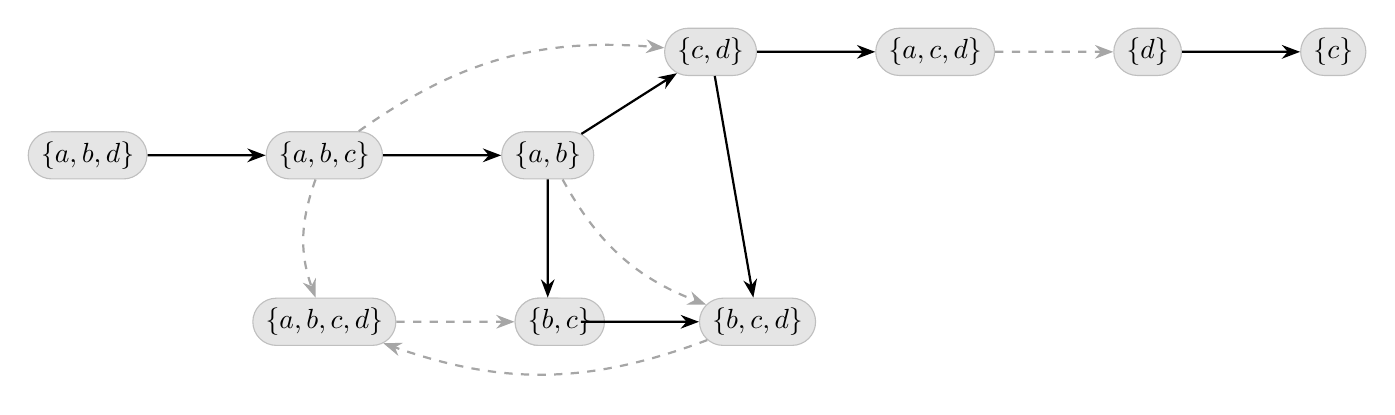
\begin{tikzpicture}[node distance=1.5cm]
  % 定义节点样式
  \tikzset{
    set node/.style={
      rounded rectangle,
      fill=gray!20,
      draw=gray!50,
      inner sep=3pt,
      minimum height=0.6cm
    },
    solid arrow/.style={
      ->,
      >=Stealth,
      line width=0.8pt
    },
    dashed arrow/.style={
      ->,
      >=Stealth,
      dashed,
      draw=gray!70,
      line width=0.8pt
    }
  }
  
  % 创建节点
  \node[set node] (abd) {$\{a,b,d\}$};
  \node[set node, right=of abd] (abc) {$\{a,b,c\}$};
  \node[set node, right=of abc] (ab) {$\{a,b\}$};
  \node[set node, above right=0.7cm and 1.5cm of ab] (cd) {$\{c,d\}$};
  \node[set node, right=of cd] (acd) {$\{a,c,d\}$};
  \node[set node, right=of acd] (d) {$\{d\}$};
  \node[set node, right=of d] (c) {$\{c\}$};
  \node[set node, below=of ab] (b) {$\{b\}$};
  \node[set node, right=of b] (bcd) {$\{b,c,d\}$};
  \node[set node, below=of abc] (abcd) {$\{a,b,c,d\}$};
  \node[set node, right=of abcd] (bc) {$\{b,c\}$};
  
  % 绘制实线箭头
  \draw[solid arrow] (abc) -- (ab);
  \draw[solid arrow] (ab) -- (cd);
  \draw[solid arrow] (ab) -- (b);
  \draw[solid arrow] (b) -- (bcd);
  \draw[solid arrow] (cd) -- (acd);
  \draw[solid arrow] (cd) -- (bcd);
  \draw[solid arrow] (abd) -- (abc);
  \draw[solid arrow] (d) -- (c);
  
  % 绘制虚线箭头
  \draw[dashed arrow] (abc) to[bend right=20] (abcd);
  \draw[dashed arrow] (ab) to[bend right=20] (bcd);
  \draw[dashed arrow] (bcd) to[bend left=20] (abcd);
  \draw[dashed arrow] (abcd) -- (bc);
  \draw[dashed arrow] (abc) to[bend left=20] (cd);
  \draw[dashed arrow] (acd) -- (d);
  
\end{tikzpicture}
\end{document}